\hypertarget{ux3053ux3093ux306bux3061ux306f-konnichiwa}{%
\section{こんにちは, konnichiwa
!}\label{ux3053ux3093ux306bux3061ux306f-konnichiwa}}

C'est après une très courte nuit dans l'avion qui nous amène de Shanghai
que nous posons pied sur l'archipel japonais, aussi appelé "la banane".
Une fois notre Japan Rail Pass en poche, des retrouvailles nous
attendent à Osaka, où nous sommes accueillis par Sorouch et Wakana.

\begin{figure}
\centering
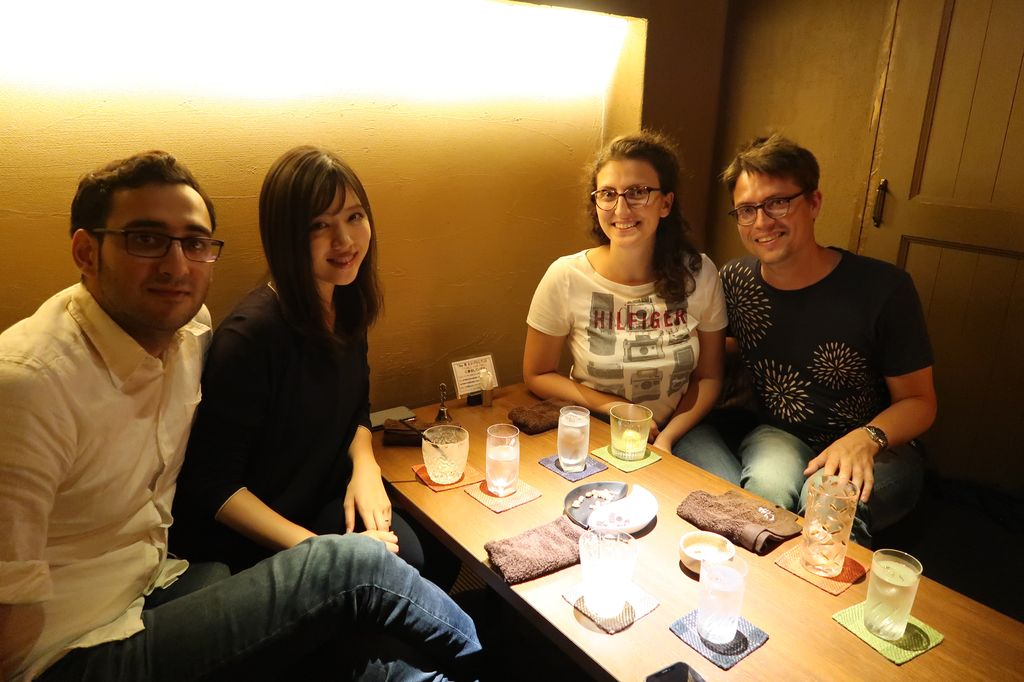
\includegraphics{images/20180625_osaka.JPG}
\caption{Nos hôtes dans le Kansai (région autour de Kyoto et Osaka),
Sorouch et Wakana, nous ont fait découvrir les spécialités d'Osaka.}
\end{figure}

Après deux courtes journées à Osaka, nous enchaînons avec un séjour dans
l'île la plus à l'ouest de l'archipel nippon, Kyushu.

Ce que nous vous raconterons bientôt, pour la suite de nos aventures au
Japon !

\emph{Florian et Elida}
